% Format teze zasnovan je na paketu memoir
% http://tug.ctan.org/macros/latex/contrib/memoir/memman.pdf ili
% http://texdoc.net/texmf-dist/doc/latex/memoir/memman.pdf
% 
% Prilikom zadavanja klase memoir, navedenim opcijama se podešava 
% veličina slova (12pt) i jednostrano štampanje (oneside).
% Ove parametre možete menjati samo ako pravite nezvanične verzije
% doktorata za privatnu upotrebu (na primer, u b5 varijanti ima smisla 
% smanjiti 
\documentclass[12pt,oneside]{memoir} 

% Paket koji definiše sve specifičnosti doktorata Matematičkog fakulteta
\usepackage[cirlat]{matfdoktorat} 

% Ovaj dokument prikazuje kako se koristi mogućnost unosa ćiriličkog
% teksta latiničkim pismom. Za to je potrebno da se koristi opcija 
% cirlat (koja je već navedena), kao i prevodilac XeLaTeX. 
% U ovoj vrsti dokumenata relevantne su sledeće opcije.

% Opcija [cirlat]:
% Sav latinički tekst na srpskom jeziku treba biti okružen sa
% \lat{...} ili \begin{latinica}...\end{latinica}.
%
% Opcija [biblatex]:
%   ako želite da koristite reference na više jezika i umesto paketa
%   bibtex da koristite BibLaTeX/Biber, dodajte opciju "biblatex" tj.
%   prethodni paket uključite pomoću: \usepackage[biblatex]{matfdoktorat}
%
% Opcija [b5paper]:
%   ako želite da napravite verziju teze u manjem (b5) formatu, navedite
%   opciju "b5paper", tj. prethodni paket uključite pomoću: 
%   \usepackage[b5paper]{matfdoktorat}. Tada ima smisla razmisliti o promeni
%   veličine slova (izmenom opcije 12pt na 11pt u \documentclass{memoir}).
%
% Naravno, opcije je moguće kombinovati.
% Npr. \usepackage[b5paper,biblatex]{matfdoktorat}

% Pomoćni paket koji generiše nasumičan tekst u kojem se javljaju sva slova
% azbuke (nema potrebe koristiti ovo u pravim disertacijama)
\usepackage[latinica]{pangrami}

% Paket koji obezbeđuje ispravni prikaz ćiriličkih italik slova kada
% se koristi pdflatex. Zakomentarisati ako na sistemu koji koristite ovaj
% paket nije dostupan ili ako ne radi ispravno.
\usepackage{cmsrb}

% Ostali paketi koji se koriste u dokumentu
\usepackage{listings} % listing programskog koda

% Datoteka sa literaturom u BibTex tj. BibLaTeX/Biber formatu
\bib{matfdoktorat-primer}

% Ime doktoranda na srpskom jeziku (obavezno uneti ćirilicom)
\autor{Петар Петровић}
% Ime doktoranda na engleskom jeziku
\author{Petar P. Petrović}
% Naslov teze na srpskom jeziku (obavezno uneti ćirilicom)
\naslov{Докторат из математике или рачунарства чији је наслов јако дугачак}
% Naslov teze na engleskom jeziku
\title{Doctoral Dissertation in Mathematics or Computer Science}
% Godina u kojoj je teza predana komisiji
\godina{2015}
% Ime i afilijacija mentora (u odabranom pismu)
\mentor{dr Mika \textsc{Mikic1}, redovan profesor\\ Univerzitet u Beogradu, Matematichki fakultet}
% Ime i afilijacija prvog člana komisije (u odabranom pismu)
\komisijaA{dr Ana \textsc{Anic1}, vanredni profesor\\ \lat{University of Disneyland}, Nedođija}
% Ime i afilijacija drugog člana komisije (u odabranom pismu)
\komisijaB{dr Laza \textsc{Lazic1}, docent\\ Univerzitet u Beogradu, Matematichki fakultet}
% Ime i afilijacija trećeg člana komisije (opciono)
% \komisijaC{}
% Ime i afilijacija četvrtog člana komisije (opciono)
% \komisijaD{}
% Datum odbrane (odkomentarisati narednu liniju i upisati datum odbrane ako je poznat)
% \datumodbrane{}

% Apstrakt na srpskom jeziku (u odabranom pismu)
\apstr{%
\pangrami
}

% Apstrakt na engleskom jeziku
\abstr{%
\pangrami

\pangrami
}

% Ključne reči na srpskom jeziku (u odabranom pismu)
\kljucnereci{analiza, geometrija, algebra, logika, rachunarstvo, astronomija}

% Ključne reči na engleskom jeziku
\keywords{analysis, geometry, algebra, logic, computer science, astronomy}

% Šira i uža oblast teze na srpskom jeziku (u odabranom pismu)
\oblast{rachunarstvo}
\uzaoblast{bioinformatika}

% Šira i uža oblast teze na engleskom jeziku
\area{computer science}
\subarea{bioinformatics}

% Univerzalna decimalna klasifikacija (UDK tj. UDC) 
% https://en.wikipedia.org/wiki/Universal_Decimal_Classification
\udk{004.415.5(043.3)}

\begin{document}
% ==============================================================================
% Uvodni deo teze
\frontmatter
% ==============================================================================
% Naslovna strana
\naslovna
% Naslovna strana na engleskom jeziku
\naslovnaen
% Strana sa podacima o mentoru i članovima komisije
\komisija
% Strana sa posvetom (u odabranom pismu)
\posveta{Mami, tati i dedi}
% Strana sa podacima o disertaciji na srpskom jeziku
\apstrakt
% Strana sa podacima o disertaciji na engleskom jeziku
\apstrakten
% Sadržaj teze
\tableofcontents*

% ==============================================================================
% Glavni deo teze
\mainmatter
% ==============================================================================

% ------------------------------------------------------------------------------
\chapter{Uvod}
% ------------------------------------------------------------------------------
\pangrami

\section{Unos c1irilichkih karaktera latinicom}

Ako se koristi \lat{Xe\LaTeX}, c1irilichki tekst se mozhe unositi
latinicom, uz korish\/c1enje dijakritichkih karaktera
(\lat{ćčšžđĆČŠŽĐ} i kombinacija karaktera \lat{nj, lj, dž, Nj, Lj} i
\lat{Dž}). Pored toga, moguc1e je koristiti i kombinacije prikazane u
tabeli \ref{fig:cirilicki_unos}, koje omoguc1avaju da se sve vreme
korisi samo engleska tastatura.

\begin{table}[ht]
  \centering
  \begin{tabular}{cc}
    c1irilichki karakter & moguc1i nachini unosa\\
    Dj & \lat{Đ, Dj, DJ}\\
    dj & \lat{đ, dj}\\
    Z1 & \lat{Ž, ZH, Zh, Z1}\\
    z1 & \lat{ž, zh, z1}\\
    C1 & \lat{Ć, C1, 'C}\\
    c1 & \lat{ć, c1, 'c}\\
    Ch & \lat{Č, Ch}\\
    ch & \lat{č, ch}\\
    D2 & \lat{Dž, DZH, Dzh, D1, D2}\\
    d2 & \lat{dž, dzh, d1, d2}\\
    Sh & \lat{Š, SH, Sh}\\
    sh & \lat{š, sh}\\
    Lj & \lat{Lj}\\
    lj & \lat{lj}\\
    Nj & \lat{Nj}\\
    nj & \lat{nj}
  \end{tabular}
  \caption{Могући начини уноса ћириличких карактера ако се користи \lat{Xe\LaTeX}}
  \label{fig:cirilicki_unos}
\end{table}

Hajde da ih sve isprobamo (ispravno c1e raditi samo ako se koristi \lat{Xe\LaTeX}):
Đ, Dj, DJ, đ, dj, Ž, ZH, Zh, Z1, ž, zh, z1, Ć, C1, 'C, ć, c1, 'c, Č,
Ch, č, ch, Dž, DZH, Dzh, D1, D2, dž, dzh, d1, d2, Š, SH, Sh, š, sh,
Lj, lj, Nj, nj.

Ako se koristi \lat{pdf\LaTeX}, c1irilichki tekst se mozhe unositi
latinicom, uz korish\/c1enje kombinacija prikazanih u tabeli
\ref{fig:cirilicki_unos_pdflatex}, koje omoguc1avaju da se sve vreme
korisi samo engleska tastatura

\begin{table}[ht]
  \centering
  \begin{tabular}{cc}
    c1irilichki karakter & moguc1i nachini unosa\\
    Dj & \lat{Dj, DJ, D1}\\
    dj & \lat{dj, d1}\\
    Z1 & \lat{ZH, Zh, Z1}\\
    z1 & \lat{zh, z1}\\
    C1 & \lat{C1}\\
    c1 & \lat{c1}\\
    Ch & \lat{Ch}\\
    ch & \lat{ch}\\
    D2 & \lat{D2}\\
    d2 & \lat{d2}\\
    Sh & \lat{SH, Sh}\\
    sh & \lat{sh}\\
    Lj & \lat{Lj}\\
    lj & \lat{lj}\\
    Nj & \lat{Nj}\\
    nj & \lat{nj}
  \end{tabular}
  \caption{Могући начини уноса ћириличких карактера ако се користи \lat{pdf\LaTeX}}
  \label{fig:cirilicki_unos_pdflatex}
\end{table}

Hajde da ih sve isprobamo:
Dj, DJ, D1, dj, d1, ZH, Zh, Z1, zh, z1, C1, c1, Ch, ch, D2, d2, SH, Sh, sh,
Lj, lj, Nj, nj

\section{Primeri korish\/c1enja klasichnih \lat{\LaTeX{}} elemenata}
% Primeri citiranja
Ovo je rechenica u kojoj se javlja citat \cite{PetrovicMikic2015}.
Josh jedan citat \cite{GuSh:243}.
% Primeri navodnika
Isprobavamo navodnike: "Rekao je da mu se javimo sutra".
% Primer referisanja na tabelu (koja se javlja kasnije)
U tabeli \ref{tbl:rezultati} koja sledi prikazani su rezultati eksperimenta.
% Primer kraćeg latiničkog teksta
{\lat Ovo je primer latiničkog teksta u tekstu na ćirilici.}
U ovoj rečenici se javlja jedna reč na {\lat latinici}.
% Primer korišćenja fusnota
Iza ove rechenice sledi fusnota.\footnote{Ovo je fusnota.}

% Primer dužeg latiničkog teksta
\begin{latinica}
  Ovo je malo duži blok teksta ispisan latničkim pismom u okviru
  ćiriličkog dokumenta. Fijuče vetar u šiblju, ledi pasaže i kuće iza
  njih i gunđa u odžacima.
\end{latinica}

% primer teksta na engleskom jeziku
\begin{english}
  This sentence is written in English. The quick, brown fox jumps over the
  lazy dog.
\end{english}

% Primer korišćenja tabele
\begin{table}
\centering
\caption{Rezultati}
\label{tbl:rezultati}
\begin{tabular}{c>{\centering}p{2cm}c}
\toprule
1 & 2 & 3\\\midrule
4 & 5 & 6\\\cmidrule(rl){1-2}
7 & 8 & 8\\
\bottomrule
\end{tabular}
\end{table}

% Primer korišćenja slike
\begin{figure}[!ht]
  \centering
  \label{fig:grafikon}
  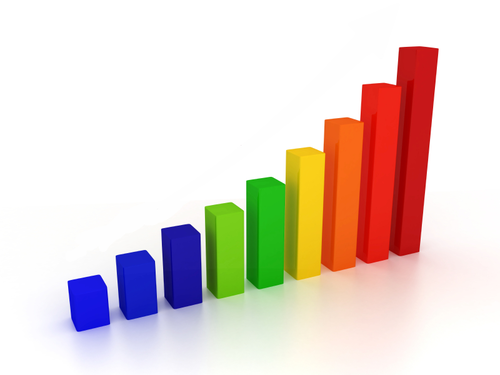
\includegraphics[width=0.5\textwidth]{graph.png}
  \caption{Grafikon}
\end{figure}


% Primer jednostavnije matematičke formule
Evo i jedan primer matematichke formule: \(e^{i\pi} + 1 = 0\).
% naravno, dozvoljeno je koristiti i dobri stari $...$ stil, ali je \(...\) 
% više u duhu LaTeX-a i ima određene prednosti (npr. jasnije poruke o greškama)

% Primer referisanja na sliku
Na slici \ref{fig:grafikon} prikazan je jedan grafikon.

% primer kompleksnije matematičke formule
\[
\int_a^b f(x)\ \mathrm{d}x \ =_{def}\ \lim_{\max{\Delta x_k \rightarrow 0}} \sum_{k=1}^n f(x_k^*)\Delta x_k
\]
% slično kao i malo pre, dozvoljeno je koristiti i $$...$$, ali \[...\] ima
% određenih prednosti


% primer referisanja na poglavlja i strane poglavlja
Vishe detalja bic1e dato u glavi \ref{chp:razrada} na strani \pageref{chp:razrada}.

U tezu mozhemo ubaciti i programski kôd.

\begin{english}
\lstset{
language=C,
basicstyle=\ttfamily,
keywordstyle=\color{blue}
}
\begin{lstlisting}
#include <stdio.h>

int main() {
   printf("Hello, world!\n");
   return 0;
}
\end{lstlisting}
\end{english}

Ovaj C program se mozhe prevesti pomoc1u prevodioca \cite{gcc}.

% primer liste
Mozhemo praviti i nabrajanja:
\begin{enumerate}
\item Analiza 1
\item Linearna algebra
\item Analitichka geometrija
\item Osnovi programiranja
\end{enumerate}

% primer nenumerisane liste
Nabrajanje mozhe biti i nenumerisano:

\begin{itemize}
\item Analiza 1
\item Linearna algebra
\item Analitichka geometrija
\item Osnovi programiranja
\end{itemize}

% primer opisne liste
Opisne liste se koriste kada se opisuje svaka od nekoliko stavki.

\begin{description}
\item[\lat{pdflatex}] - klasichni prevodilac za \lat{\LaTeX} koji
  koristi specifichne fontove.
\item[\lat{xelatex}] - moderniji prevodilac za \lat{\LaTeX} koji
  koristi \lat{OpenType} i \lat{TrueType} fontove.
\end{description}

\pangrami

% ------------------------------------------------------------------------------
\chapter{Razrada}
\label{chp:razrada}

% ------------------------------------------------------------------------------

\pangrami

\pangrami

% ------------------------------------------------------------------------------
\chapter{Zakljuchak}
% ------------------------------------------------------------------------------
\pangrami

\pangrami

% ------------------------------------------------------------------------------
% Literatura
% ------------------------------------------------------------------------------
\literatura

% ==============================================================================
% Završni deo teze i prilozi
\backmatter
% ==============================================================================

% ------------------------------------------------------------------------------
% Biografija doktoranda
\begin{biografija}
  \textbf{Vuk Stefanovic1 Karadzhic1} (\emph{Trshic1,
    26. oktobar/6. novembar 1787. — Bech, 7. februar 1864.}) bio je
  srpski filolog, reformator srpskog jezika, sakupljach narodnih
  umotvorina i pisac prvog rechnika srpskog jezika.  Vuk je
  najznachajnija lichnost srpske knjizhevnosti prve polovine XIX
  veka. Stekao je i nekoliko pochasnih doktorata.  Uchestvovao je u
  Prvom srpskom ustanku kao pisar i chinovnik u Negotinskoj krajini, a
  nakon sloma ustanka preselio se u Bech, 1813. godine. Tu je upoznao
  Jerneja Kopitara, cenzora slovenskih knjiga, na chiji je podsticaj
  krenuo u prikupljanje srpskih narodnih pesama, reformu c1irilice i
  borbu za uvođenje narodnog jezika u srpsku knjizhevnost. Vukovim
  reformama u srpski jezik je uveden fonetski pravopis, a srpski jezik
  je potisnuo slavenosrpski jezik koji je u to vreme bio jezik
  obrazovanih ljudi. Tako se kao najvazhnije godine Vukove reforme
  istichu 1818., 1836., 1839., 1847. i 1852.
\end{biografija}
% ------------------------------------------------------------------------------


% Prilog 1: Izjava o autorstvu
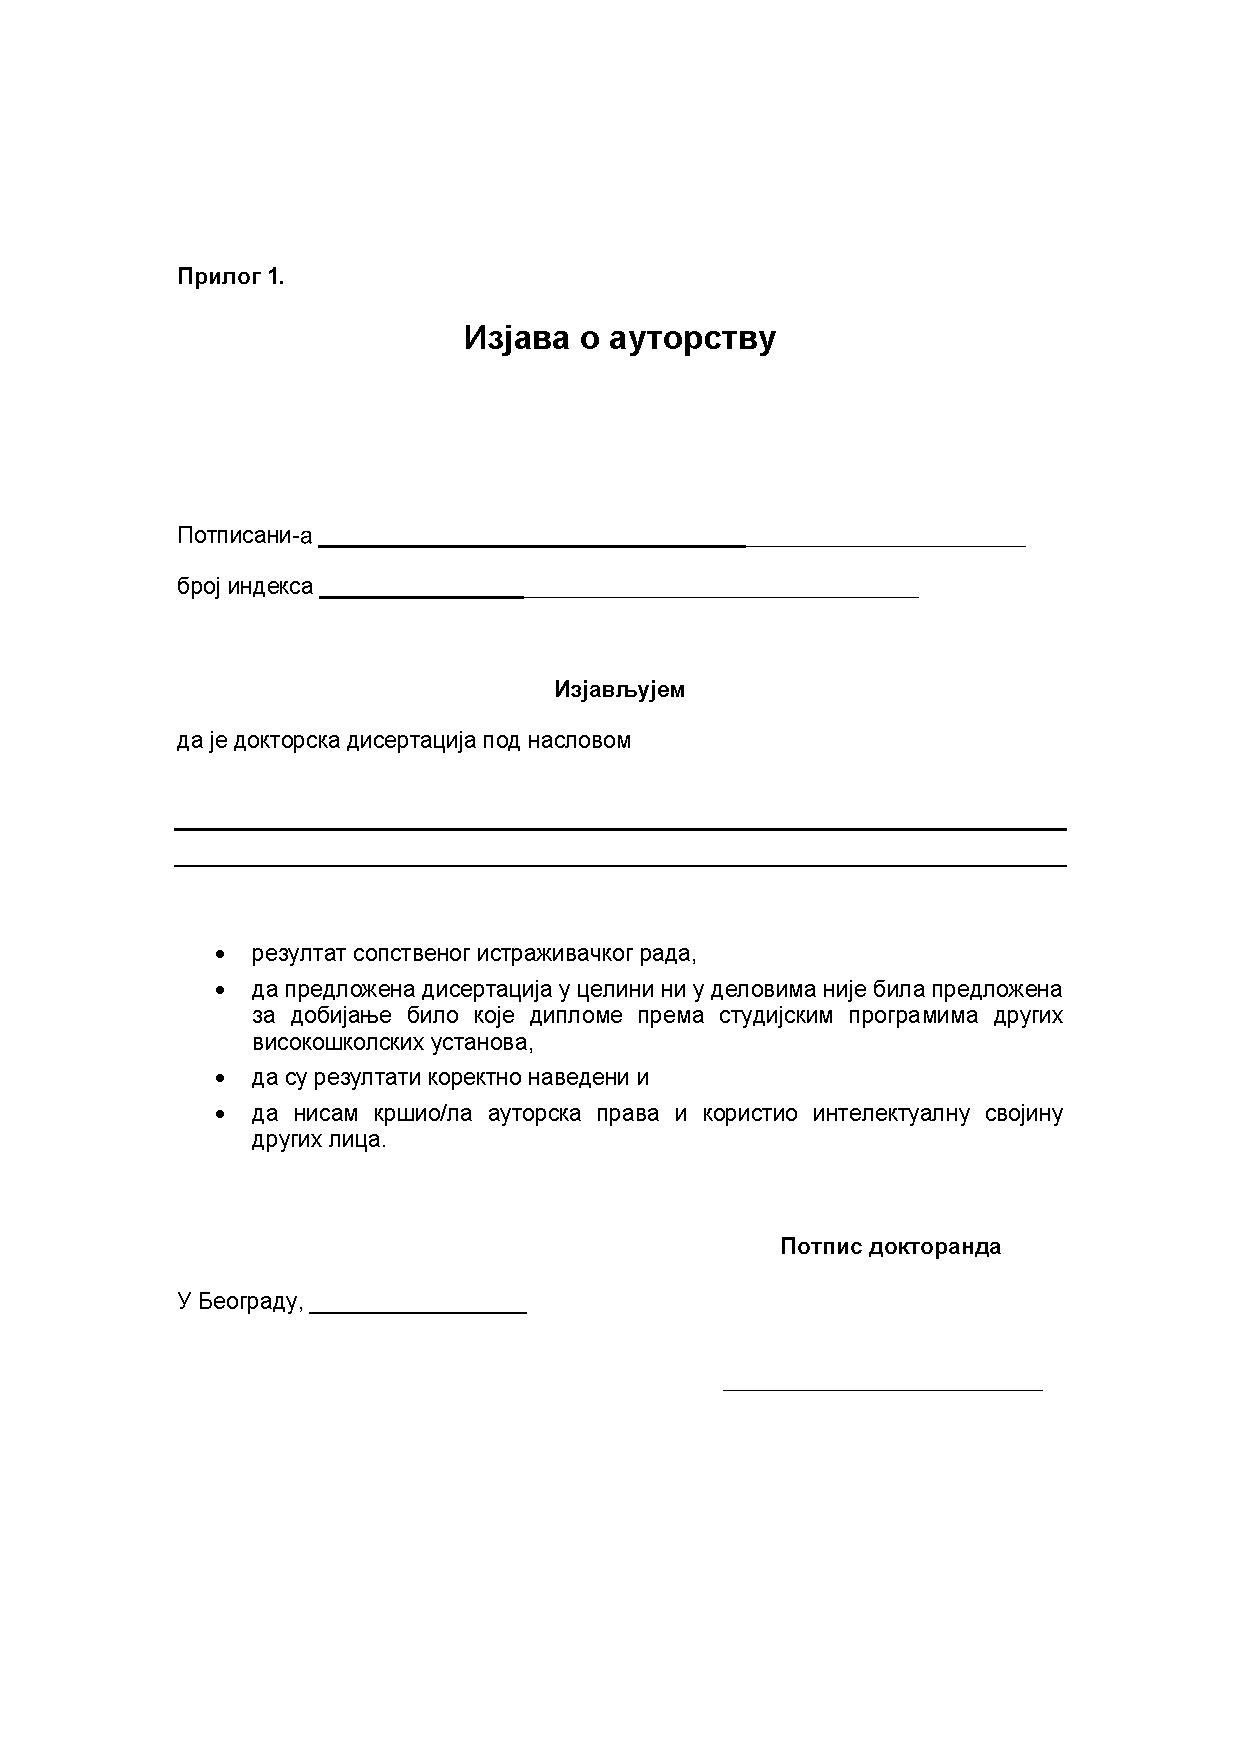
\includepdf{_Prilog1.pdf}
% Prilog 2: Izjava o istovetnosti štampane i elektronske verzije doktorskog rada
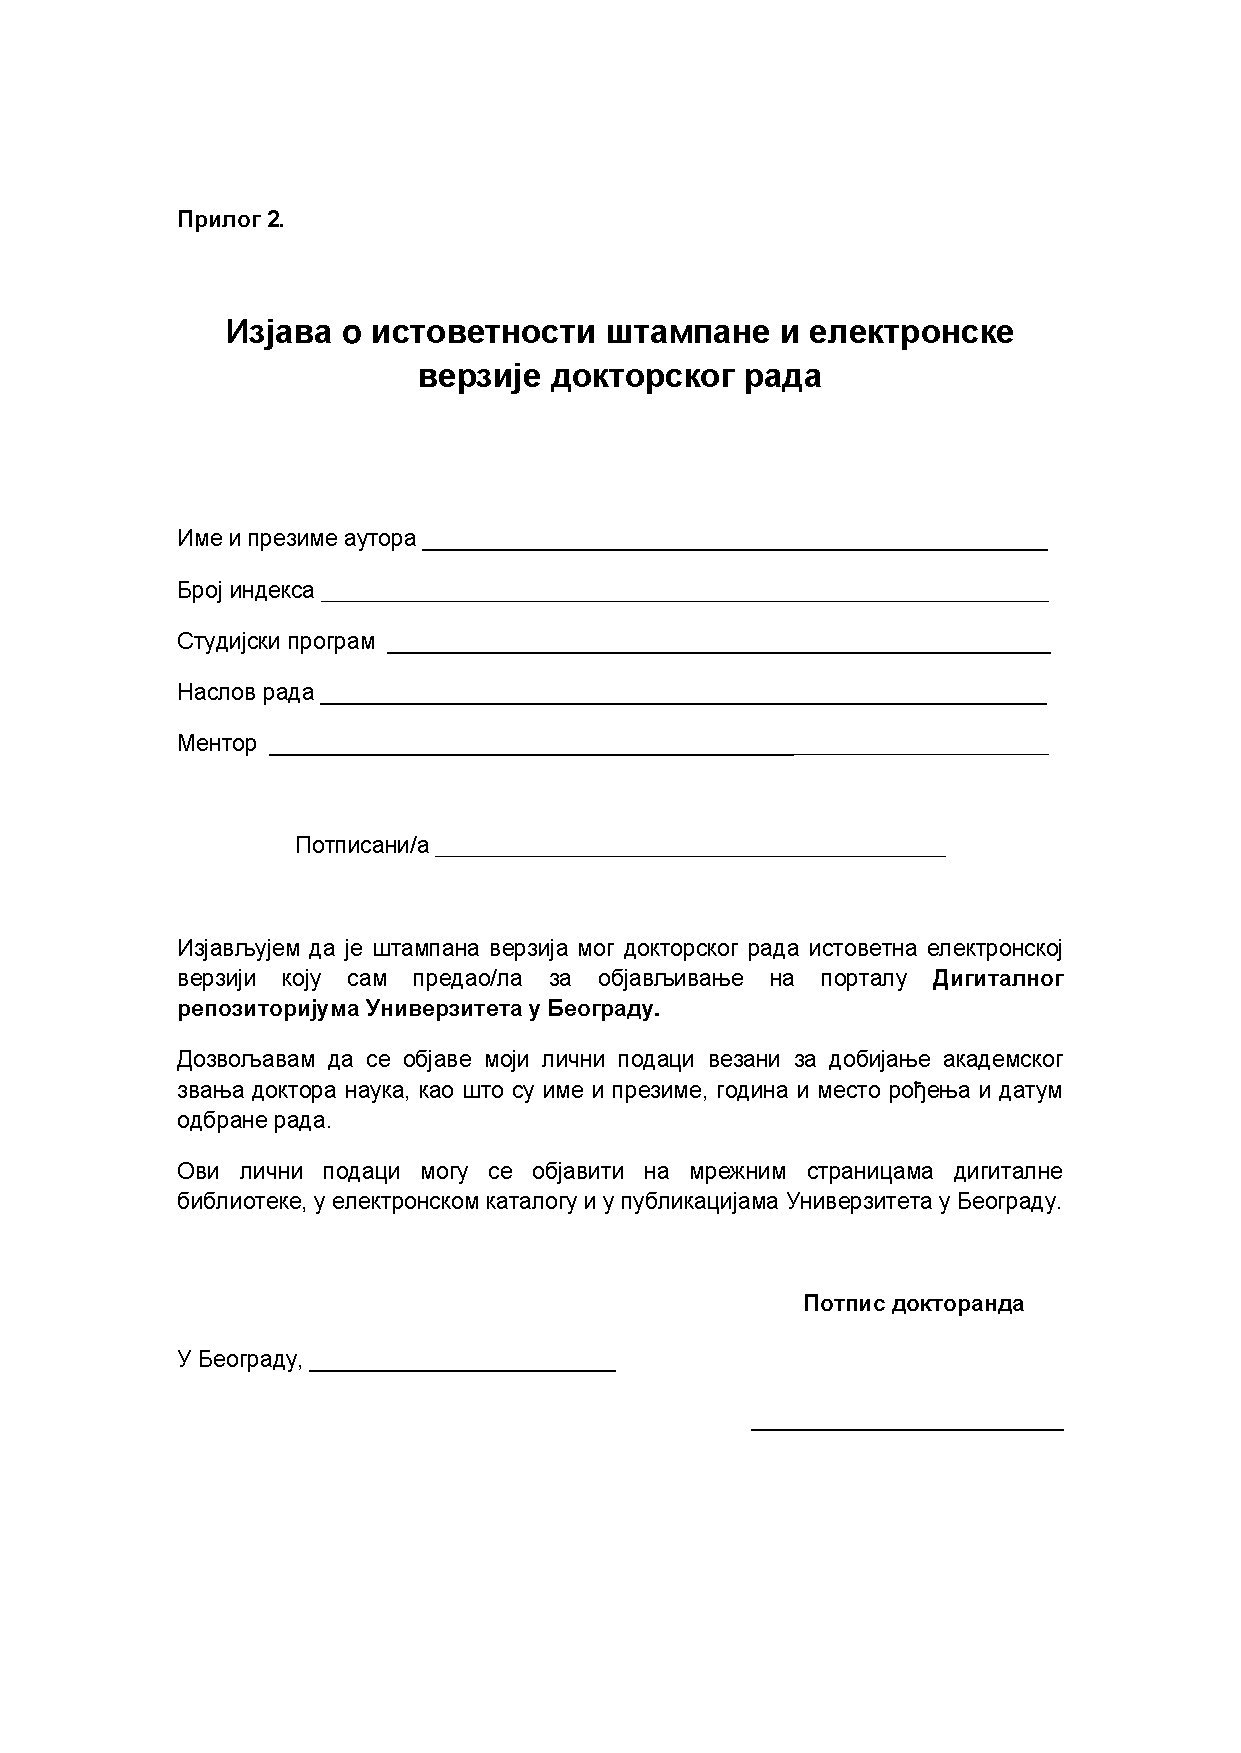
\includepdf{_Prilog2.pdf}
% Prilog 3: Izjava o korišćenju
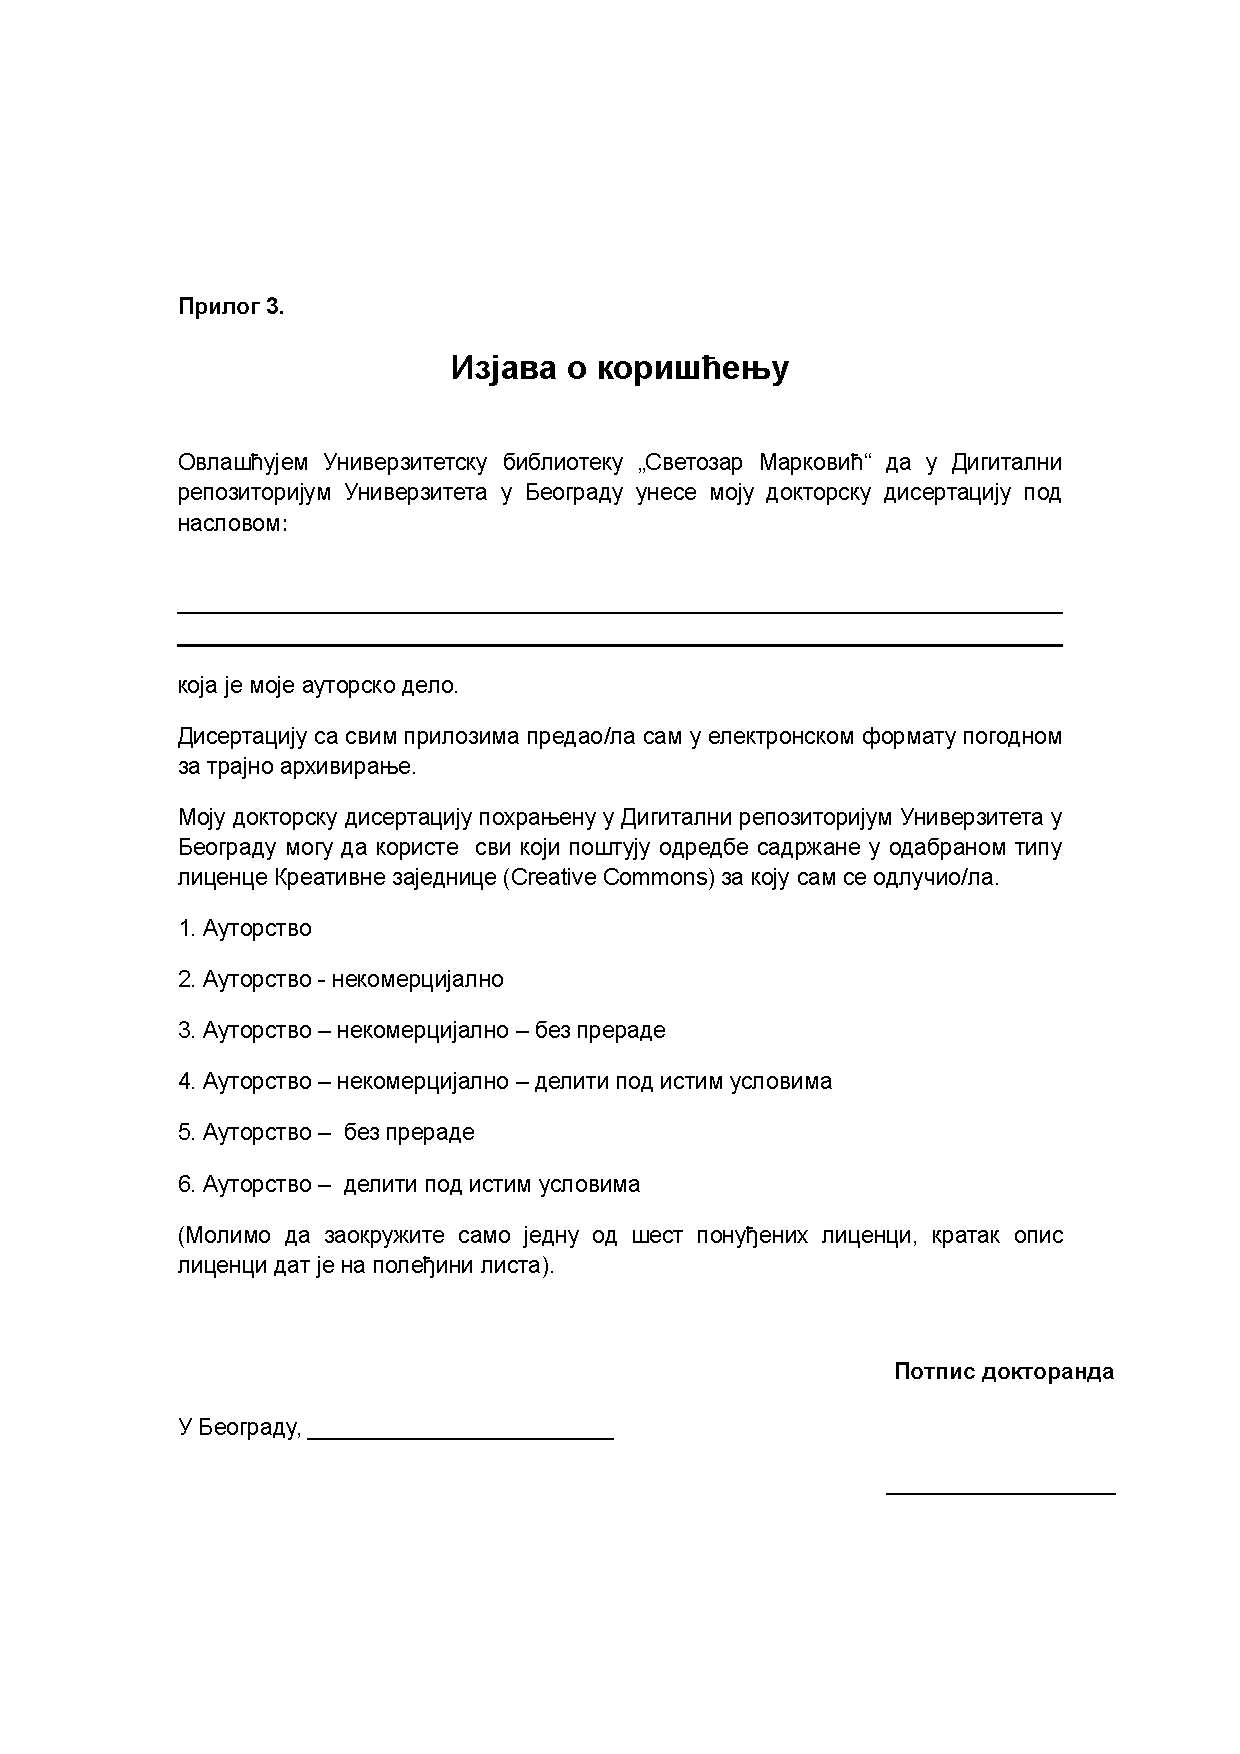
\includepdf{_Prilog3.pdf}

\end{document}